\subsection{Overview}
	Computer simulation is getting popular in the field of science. Individuals tackle diverse experimental issues using computer control through simulating artificial testing environments. They use these simulated environments to test scientific models in order to prove or disprove their feasibility and correctness.
	 
	Today's high machine power gives people the capacity to simulate environments at a rate much quicker than any real environment, thus any experiment carried out in the simulated medium would provide results minutes, hours, days and often weeks, months and years ahead of what the same experiment would provide if executed in the real world.
	
	One of the frameworks or systems that are best considered using a computer simulation is a traffic network. It is typical to experiment with traffic networks in a computer-simulated environment because experimenting with traffic in the real environment is impractical. 

\subsection{Simulation models}
	A typical classification method for simulation models is based on the variability content that represents the deterministic nature of simulation that represents the static or dynamic characteristics of simulation. Regarding how frequent the activity of the traffic network is updated and the statistics on traffic performance is collected, the most frequently used classification method is based on the details a model intends to simulate, namely, microscopic or macroscopic modelling.
\subsubsection{Microscopic modelling}
	Microscopic simulation modelling methods are based on car-following and lane-changing theories, which can represent the traffic operations and vehicle/driver behaviours in detail. The car-following theory describes the longitudinal movement of vehicles. The classical car-following approach is quite straightforward, i.e., each vehicle attempts to advance at its desired speed while maintaining a safe following distance from the vehicle ahead\cite{rathi1986freesim}. Microscopic simulation modelling incorporates queuing analysis, shock-wave analysis, and other analytical techniques.
\subsubsection{Macroscopic modelling}
	Macroscopic models do not consider car-following behaviour in detail, but instead model traffic as an aggregate fluid flow. To better understand the collective behaviour of traffic and analyse flow conditions in a dynamic fashion, continuum models, either simple or high-order, are usually employed in macroscopic simulation modelling. The simple continuum model consists of a continuity equation representing the relationship between the speed, density, and flow generation rate \cite{ross1988some}. Although the existing high-order models look promising, they have not as yet proved truly superior to the simple continuum models at least in medium-to-congested flow conditions\cite{michalopoulos1991enhancement}
\subsection{Comparison of different traffic simulation packages}
	We will briefly review the following well known and widely used simulation packages;
	
	\begin{itemize}
		\item Simulation of Urban Mobility (SUMO)
		\item Quadstone Paramics Modeller
		\item Aimsun
	\end{itemize}

\subsubsection{Simulation of Urban Mobility (SUMO)}
	Simulation of Urban Mobility (SUMO) is an open source, very compact, microscopic road traffic simulation package designed to handle large road networks\cite{EM1}.
	\begin{center}
	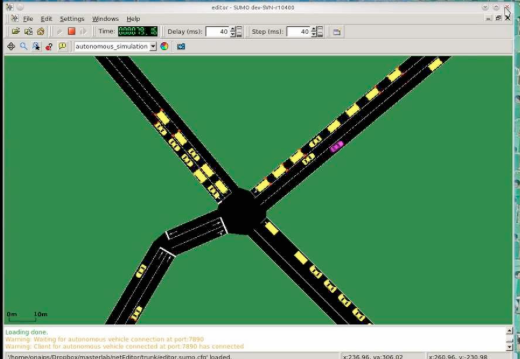
\includegraphics[scale=0.3]{./images/SUMO.png}
	\end{center}
	The simulation platform SUMOs features include:
	\begin{itemize}
		\item Microscopic simulation – vehicles and public transport are modelled explicitly.
		\item Simulation of multi-modal traffic, e.g. Vehicles, public transport, and pedestrians.
		\item Time schedules of traffic lights can be imported or generated automatically by SUMO.
		\item No artificial limitations in network size and number of simulated vehicles \cite{EM1}.
	\end{itemize}

	Traffic networks and associated vehicle patterns can be created manually in XML, using an automatic network generator and can also import networks created in other traffic simulation applications.
	
	SUMO includes simulation output through generating output files. The output files contains the following;
	
	\begin{itemize}
		\item Network state dump of a certain point of time in the simulation.
		\item Lane dump of a certain point of time in the simulation
		\item Vehicle trip information
		\item Traffic lights description and how their pattern affected the traffic flow.
	\end{itemize}
	
\subsubsection{Quadstone Paramics Modeller}
	
	Quadstone Paramics is a standard suite of microscopic simulation tools, which provides powerful, integrated platform for modelling the entire scope of real world traffic and transportation issues \cite{EM3}.
	\begin{center}
	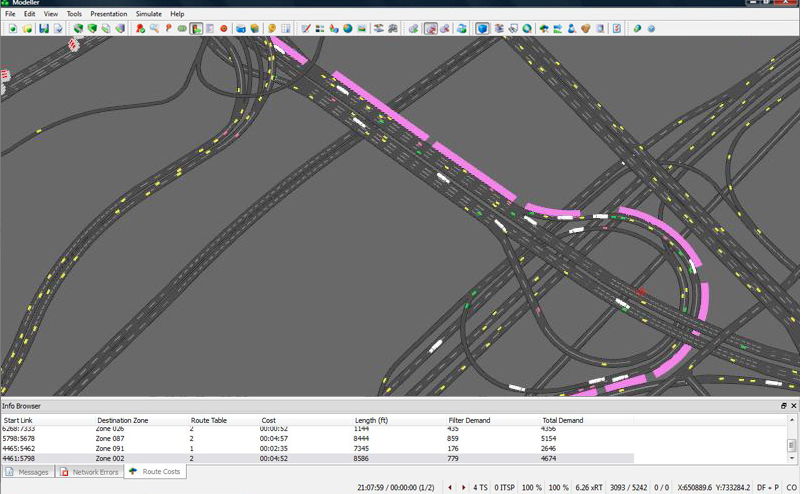
\includegraphics[scale=0.3]{./images/QPM.png}
	\end{center}
	
	Paramics Modeller produces a simulation that shows representation the traffic network, as well as public transport and vehicles \cite{EM3}.
	
	The output this package included tools to statistically represent what is happening in the simulated traffic network. The measurements included in the software applications include queuing patterns, peaks and troughs in demand, speed, density, line of sight, journey time, etc. In addition, the user could calibrate the model using all these tools during run time.
	
	In creating traffic networks and associated vehicle patterns it uses an automatic network generation wizard (that generated only a simple two zone network in the demo version) - apparently in the full version of the application a user could automatically create a traffic network using the wizard, and then further customize it using the graphical network editor available.
	
\subsubsection{Aimsun}
	Aimsun is an integrated transport modelling software, It is used to improve road infrastructure, reduce emissions, cut congestion and design urban environments for vehicles and pedestrians. The Aimsun hybrid simulator offers simultaneous microscopic and mesoscopic simulation, combining an event-based mesoscopic model for large areas with a more detailed time-sliced micro-simulator for smaller areas that require a finer level of detail \cite{EM2}.
The hybrid simulator features the following:
	\begin{itemize}
		\item Demand definition using O/D matrices or traffic states
		\item Unified statistics collection
		\item Hybrid simulator applicable to sub-networks
		\item Dynamic traffic assignment based on dynamic user equilibrium
		\item Traffic management
	\end{itemize}
	
	Traffic networks and associated vehicles are created by manually drawing of the traffic network using the available graphical network editor.
	
	Aimsun simulation output includes more than 20 different view styles for graphical representation of statistical information about the traffic and the events occurring in the ongoing simulation of the traffic network. However, we were not able to investigate them in the demo version of the software application.
	
	\begin{center}
	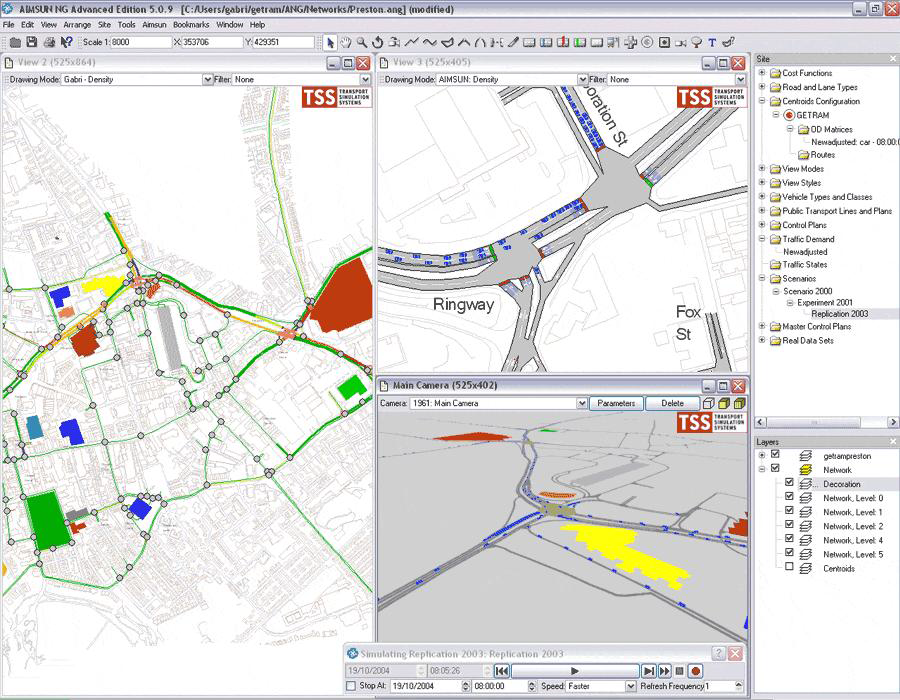
\includegraphics[scale=0.3]{./images/aimsun.png}
	\end{center}
	
	Aimsun traffic simulation package, illustrates how multiple views are used to capture different points of interest in a traffic network. Each viewpoint has its own angle, representation and graphics quality settings. \cite{EM2}.
	
\subsubsection{CPU and Memory performance}
	
		\begin{center}
		\begin{tabular}{| l | p{2.5cm} | p{2.5cm} | p{2.5cm} |}
			\hline
					& SUMO	& Paramics Modeller & Aimsun	\\ \hline
			CPU Memory	&	5-17\% depending on the number of vehicles currently running	& Constant 50\%	& 25-40\% depending on number of vehicles and scenario	\\ \hline
			Memory Usage &	12-16MB depending on the traffic network	& 40-140MB depending on network and graphic model used	& 30-40MB depending on traffic network	\\
			\hline
		\end{tabular}
		\end{center}